\subsection{System Evaluation}~\label{exp:sys_eval}
We evaluate the proposed framework from three perspectives. We first examine how the confidence threshold $\tau$ influences the trade-off between task performance and user feedback. We then compare the proposed query strategy with representative baselines under identical task settings. Finally, we analyze the computational scalability of the method as the symbolic state space increases.

\subsubsection{Threshold Ablation}~\label{exp:sys_threshold}
We first evaluate the effect of the confidence threshold $\tau$ on system performance. Fig.~\ref{fig:sys_tau} and Table~\ref{tab:sys_tau} report the resulting success rate, execution steps, and number of user queries across different threshold values.


\begin{figure*}[t!]
    \centering
    \begin{subfigure}[t]{0.40\textwidth}
        \centering
        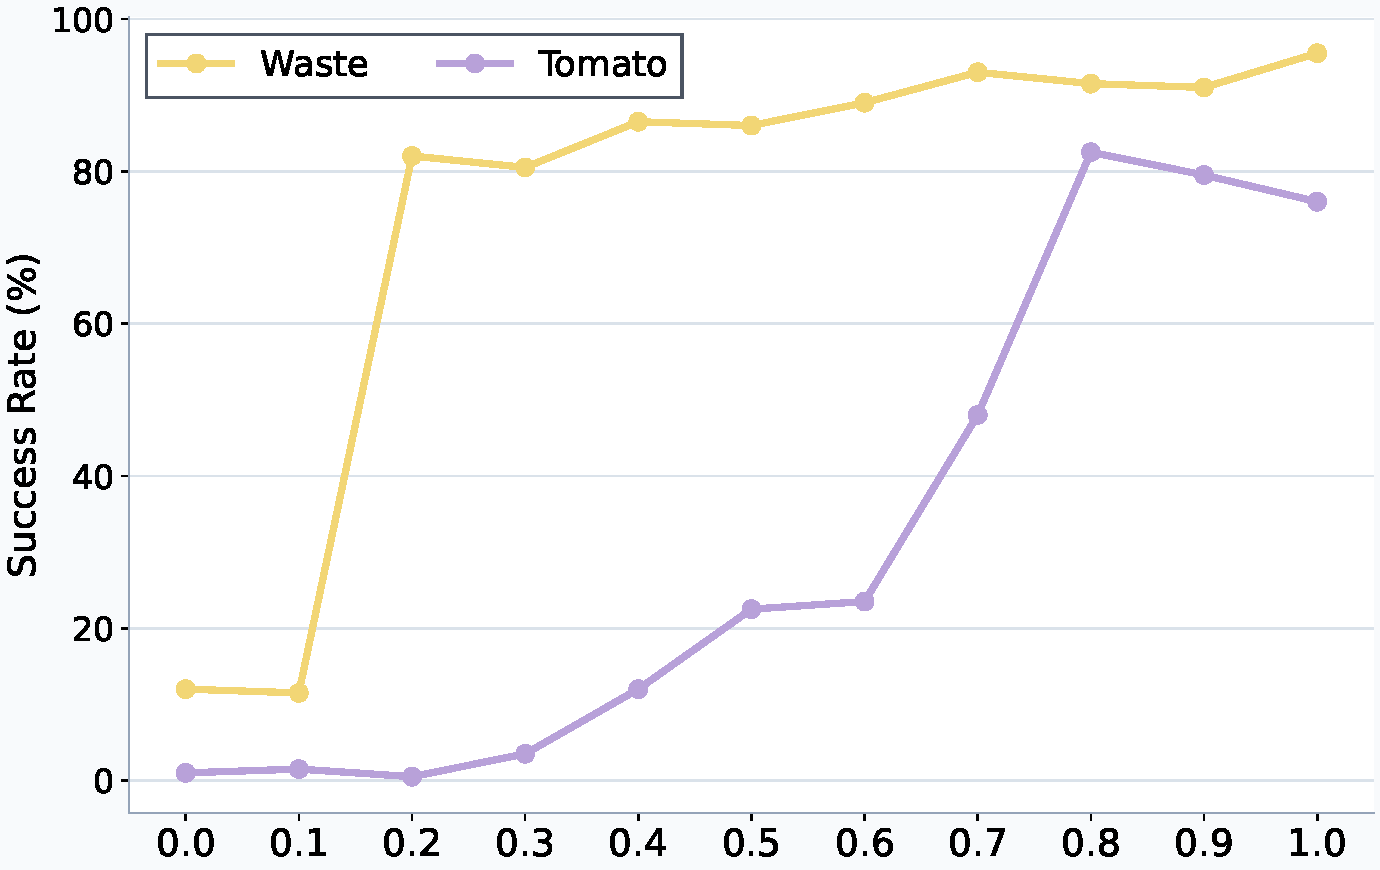
\includegraphics[width=\linewidth]{figures/system_eval/fig_thres_success_rate.pdf}
        \caption{Success rate}
        \label{fig:sys_tau_success}
    \end{subfigure}
    \hspace{0.03\textwidth}
    \begin{subfigure}[t]{0.40\textwidth}
        \centering
        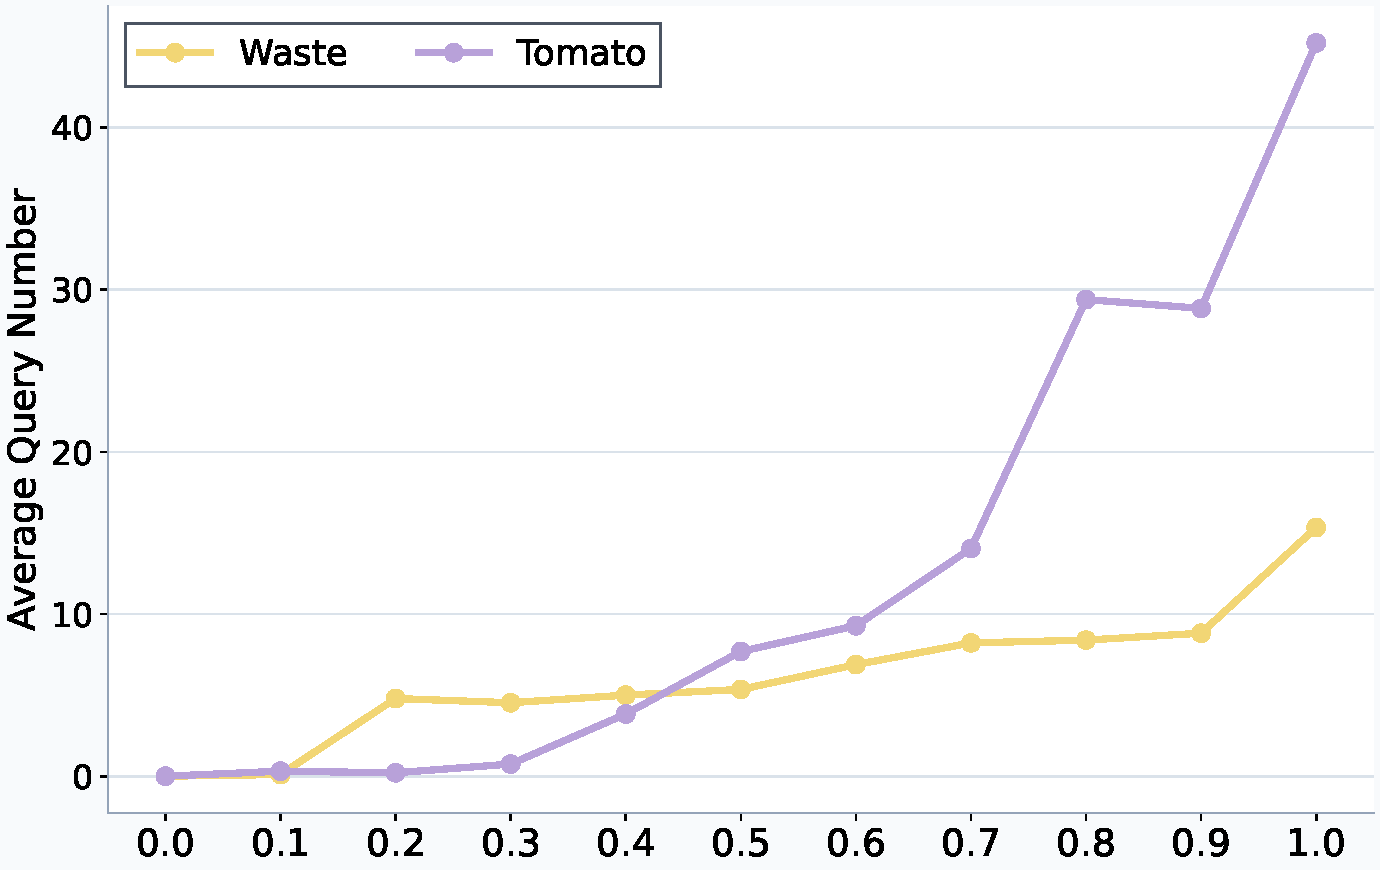
\includegraphics[width=\linewidth]{figures/system_eval/fig_thres_average_question.pdf}
        \caption{Average queries}
        \label{fig:sys_tau_queries}
    \end{subfigure}
    \vspace{0.4em}

    \begin{subfigure}[t]{0.40\textwidth}
        \centering
        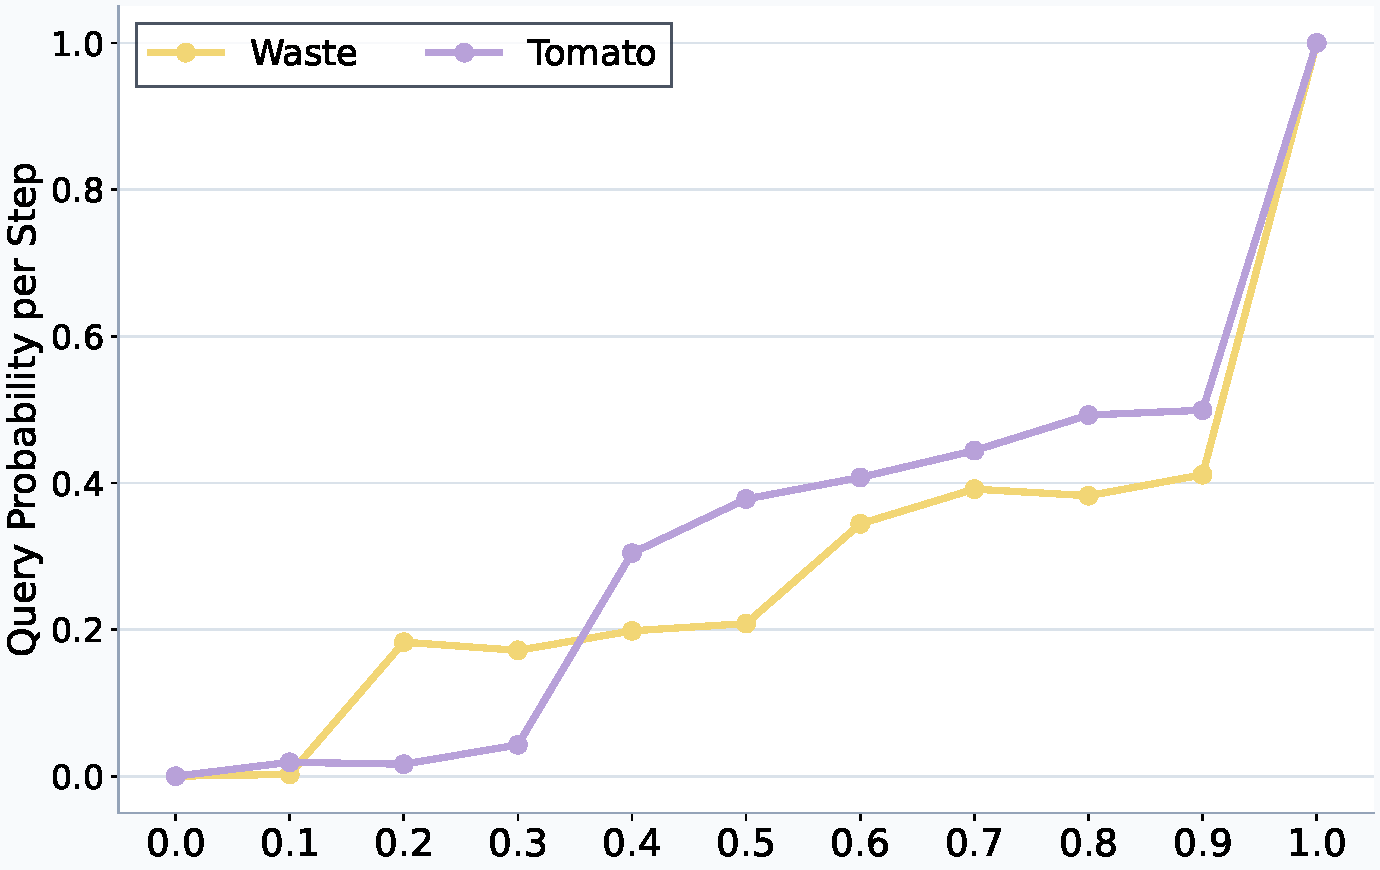
\includegraphics[width=\linewidth]{figures/system_eval/fig_thres_query_probability_per_step.pdf}
        \caption{Query rate}
        \label{fig:sys_tau_query_prob}
    \end{subfigure}
    \hspace{0.03\textwidth}
    \begin{subfigure}[t]{0.40\textwidth}
        \centering
        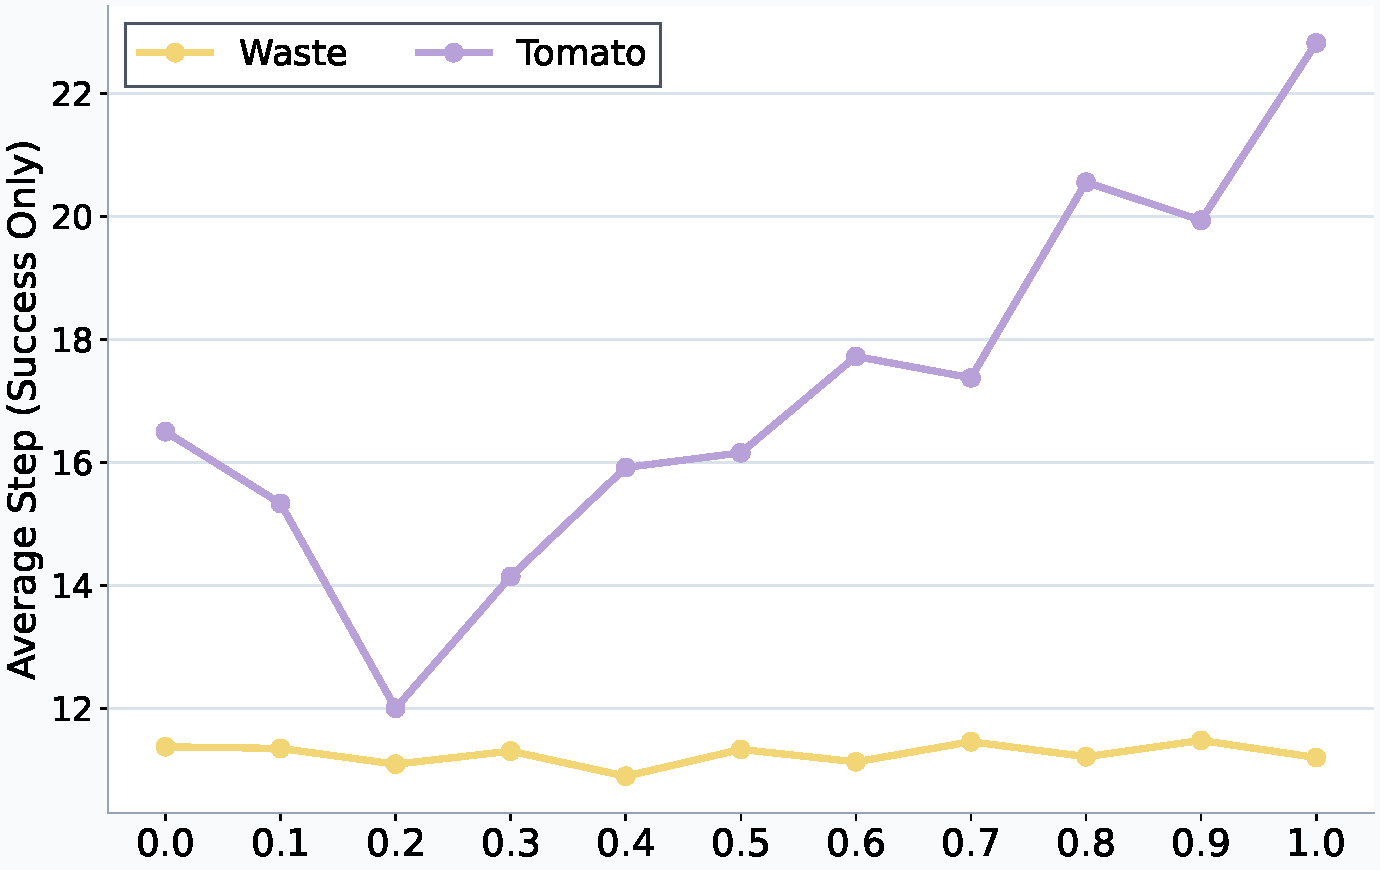
\includegraphics[width=\linewidth]{figures/system_eval/fig_thres_average_step_success_only.pdf}
        \caption{Planning length}
        \label{fig:sys_tau_steps}
    \end{subfigure}
    \caption{Effect of the confidence threshold $\tau$ on system behavior. (a) Task success rate. (b) Average number of questions per episode. (c) Query probability per execution step. (d) Planning length for successful runs. Increasing $\tau$ generally increases feedback, but very high thresholds can add interaction without improving success.}
    \label{fig:sys_tau}
\end{figure*}

\begin{table*}[t]
\centering
\caption{Threshold sensitivity for all evaluated values of $\tau$. Success rates are percentages. Query counts are average questions per episode, query rate is the fraction of execution steps with at least one question, and average steps are computed over successful runs. Each domain-threshold cell aggregates $200$ episodes.}
\label{tab:sys_tau}
\footnotesize
\setlength{\tabcolsep}{2pt}
\begin{tabular*}{\textwidth}{@{\extracolsep{\fill}}lcccccccc}
\toprule
\multirow{2}{*}{$\boldsymbol{\tau}$} & \multicolumn{4}{c}{\textbf{Waste Sorting}} & \multicolumn{4}{c}{\textbf{Tomato Harvesting}} \\
\cmidrule(lr){2-5}\cmidrule(lr){6-9}
& \textbf{Success Rate (\%)} & \textbf{Avg. Queries} & \textbf{Query Rate} & \textbf{Avg. Steps} & \textbf{Success Rate (\%)} & \textbf{Avg. Queries} & \textbf{Query Rate} & \textbf{Avg. Steps} \\
\midrule
0.0 & 12.0 & 0.0 & 0.00 & 11.4 & 1.0 & 0.0 & 0.00 & 16.5 \\
0.1 & 11.5 & 0.1 & 0.00 & 11.3 & 1.5 & 0.3 & 0.02 & 15.3 \\
0.2 & 82.0 & 4.8 & 0.18 & 11.1 & 0.5 & 0.2 & 0.02 & 12.0 \\
0.3 & 80.5 & 4.5 & 0.17 & 11.3 & 3.5 & 0.8 & 0.04 & 14.1 \\
0.4 & 86.5 & 5.0 & 0.20 & 10.9 & 12.0 & 3.8 & 0.30 & 15.9 \\
0.5 & 86.0 & 5.3 & 0.21 & 11.3 & 22.5 & 7.7 & 0.38 & 16.2 \\
0.6 & 89.0 & 6.9 & 0.34 & 11.1 & 23.5 & 9.3 & 0.41 & 17.7 \\
0.7 & 93.0 & 8.2 & 0.39 & 11.5 & 48.0 & 14.0 & 0.44 & 17.4 \\
0.8 & 91.5 & 8.4 & 0.38 & 11.2 & 82.5 & 29.4 & 0.49 & 20.6 \\
0.9 & 91.0 & 8.8 & 0.41 & 11.5 & 82.5 & 28.1 & 0.49 & 19.5 \\
1.0 & 95.5 & 15.3 & 1.00 & 11.2 & 84.0 & 48.3 & 1.00 & 23.2 \\
\bottomrule
\end{tabular*}
\end{table*}

The results show that the two domains respond differently to the confidence threshold. In waste sorting, performance improves rapidly once a small amount of uncertainty is resolved, increasing from $11.5\%$ at $\tau=0.1$ to $82.0\%$ at $\tau=0.2$. Because task success primarily depends on identifying the correct waste category, additional feedback provides limited benefit once the category is determined. In contrast, tomato harvesting involves a longer sequence of dependent decisions, including navigation, detection, picking, scanning, and execution. Unresolved uncertainty can therefore propagate through multiple stages of the task, causing performance to remain low at small threshold values. Success increases substantially only at higher thresholds and reaches $82.5\%$ at $\tau=0.8$.

Increasing $\tau$ consistently increases interaction because the planner requests feedback for a larger fraction of uncertain beliefs. This trend is reflected in both the average number of queries and the query rate. However, the additional interaction does not always translate into proportional gains in task success. In tomato harvesting, increasing the threshold from $\tau=0.8$ to $\tau=1.0$ increases the average number of queries from $29.4$ to $48.3$ and the query rate from $0.49$ to $1.00$, while success changes only slightly from $82.5\%$ to $84.0\%$. This suggests that over-querying can introduce unnecessary interaction without substantially improving downstream decisions. In waste sorting, by contrast, the simpler category-assignment structure benefits from high confidence and reaches $95.5\%$ at $\tau=1.0$. Based on the cross-domain trade-off between success and interaction cost, we use $\tau=0.8$ in the remaining experiments.



\subsubsection{Baseline Comparison}~\label{exp:sys_baseline}
We next compare the proposed query strategy with representative alternatives. \textbf{All} requests feedback whenever multiple frontier hypotheses remain, regardless of the current confidence level. \textbf{No} performs autonomous execution without user feedback. \textbf{Random} selects queries uniformly at random. \textbf{KnowNo}~\cite{ren2023robots} is a GPT-4o-based action-query baseline~\cite{achiam2023gpt}. In contrast, \textbf{Ours} selectively requests state-level feedback based on belief confidence and expected information gain. All methods are evaluated under identical task settings using $\tau=0.8$.


We note that \textbf{All} is not equivalent to setting $\tau=1.0$. The \textbf{All} policy requests feedback whenever multiple frontier hypotheses remain, whereas $\tau=1.0$ continues querying until complete confidence is achieved. Consequently, \textbf{All} may terminate querying even when uncertainty remains, while $\tau=1.0$ attempts to eliminate all uncertainty before acting.


\begin{figure*}[t!]
    \centering
    \begin{subfigure}[t]{0.40\textwidth}
        \centering
        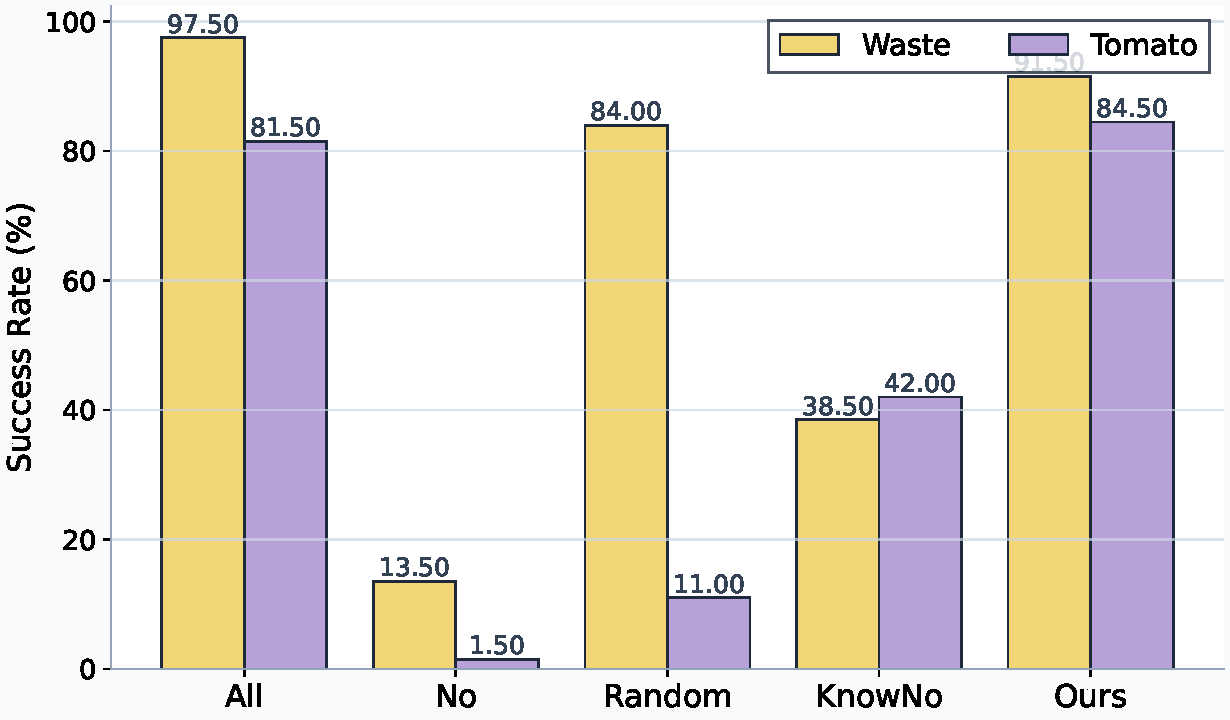
\includegraphics[width=\linewidth]{figures/system_eval/fig_ablation_success_rate.pdf}
        \caption{Success rate}
        \label{fig:sys_baseline_success}
    \end{subfigure}
    \hspace{0.03\textwidth}
    \begin{subfigure}[t]{0.40\textwidth}
        \centering
        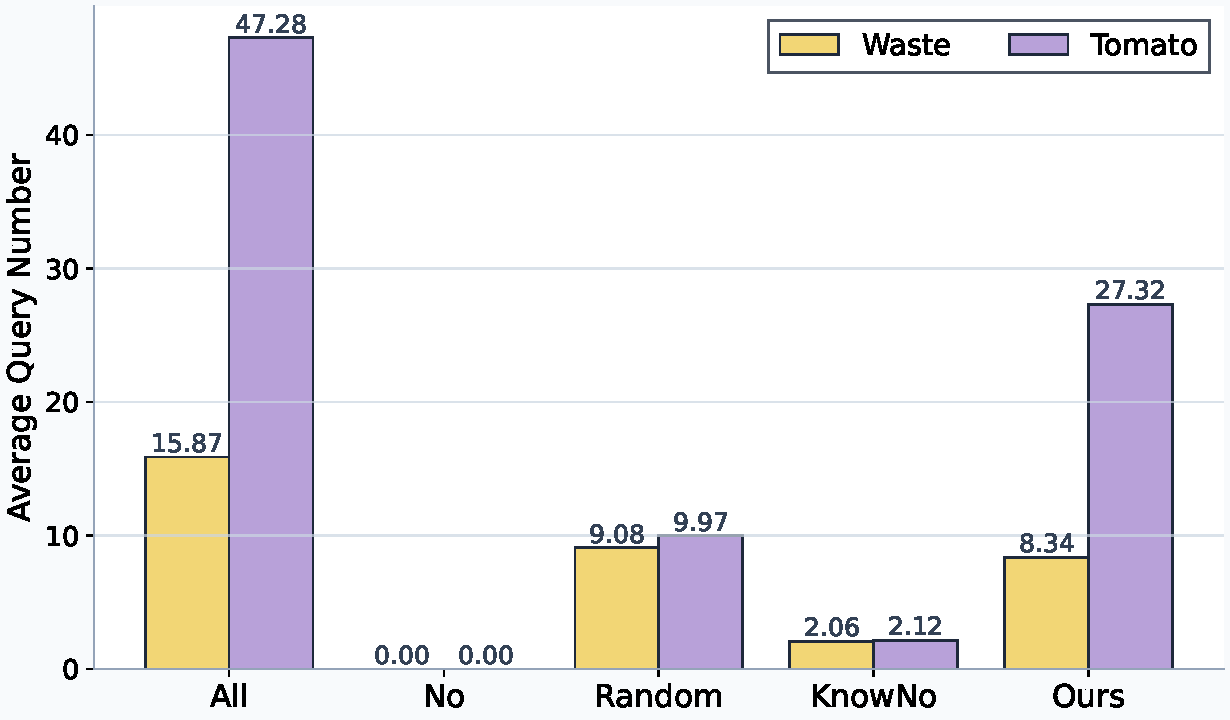
\includegraphics[width=\linewidth]{figures/system_eval/fig_ablation_average_question.pdf}
        \caption{Average queries}
        \label{fig:sys_baseline_queries}
    \end{subfigure}
    \vspace{0.4em}

    \begin{subfigure}[t]{0.40\textwidth}
        \centering
        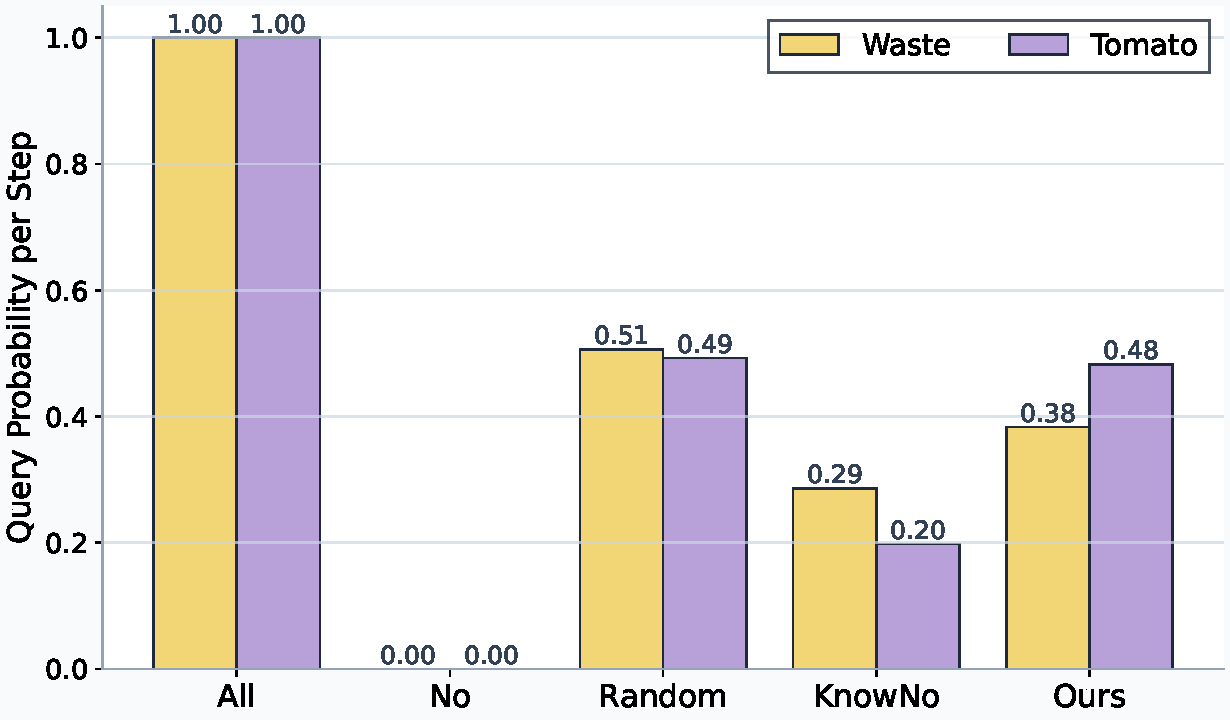
\includegraphics[width=\linewidth]{figures/system_eval/fig_ablation_query_probability_per_step.pdf}
        \caption{Query rate}
        \label{fig:sys_baseline_query_rate}
    \end{subfigure}
    \hspace{0.03\textwidth}
    \begin{subfigure}[t]{0.40\textwidth}
        \centering
        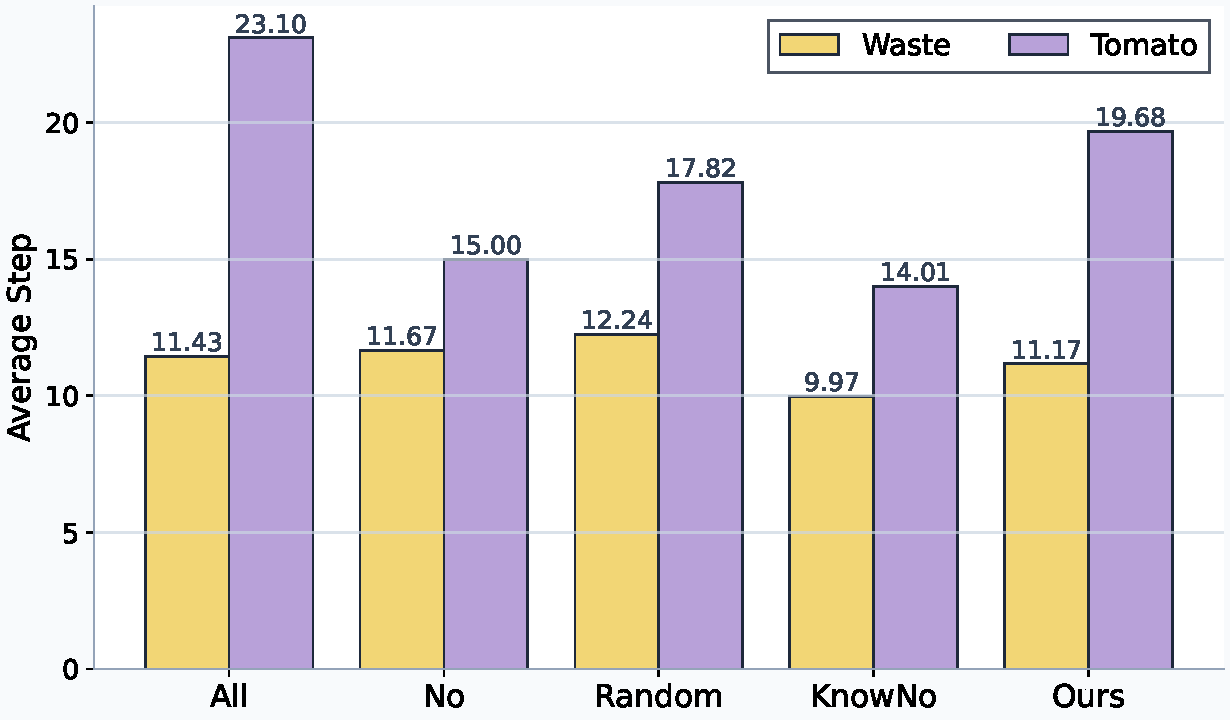
\includegraphics[width=\linewidth]{figures/system_eval/fig_ablation_average_step_success_only.pdf}
        \caption{Planning length}
        \label{fig:sys_baseline_steps}
    \end{subfigure}
    \caption{Baseline comparison at $\tau=0.8$. (a) Task success rate. (b) Average number of questions per episode. (c) Query rate, computed as the fraction of execution steps in which at least one question is asked. (d) Planning length. The proposed policy preserves high task success while asking substantially fewer questions than dense supervision.}
    \label{fig:sys_baseline}
\end{figure*}

\begin{table*}[t]
\centering
\caption{Baseline comparison at $\tau=0.8$. Average queries and query rate are computed over all episodes, while average steps are computed over successful runs.}
\label{tab:system_eval}
\footnotesize
\setlength{\tabcolsep}{2pt}
\begin{tabular*}{\textwidth}{@{\extracolsep{\fill}}lcccccccc}
\toprule
\multirow{2}{*}{\textbf{Condition}} & \multicolumn{4}{c}{\textbf{Waste Sorting}} & \multicolumn{4}{c}{\textbf{Tomato Harvesting}} \\
\cmidrule(lr){2-5}\cmidrule(lr){6-9}
& \textbf{Success Rate (\%)} & \textbf{Avg. Queries} & \textbf{Query Rate} & \textbf{Avg. Steps} & \textbf{Success Rate (\%)} & \textbf{Avg. Queries} & \textbf{Query Rate} & \textbf{Avg. Steps} \\
\midrule
\textbf{All}    & \textbf{97.5} & 15.9 & 1.00 & 11.4 & 81.5 & 47.3 & 1.00 & 23.1 \\
\textbf{No}     & 13.5 & 0.0  & 0.00 & 11.7 & 1.5  & 0.0  & 0.00 & 15.0 \\
\textbf{Random} & 90.0 & 7.9  & 0.39 & 12.7 & 10.0 & 8.9 & 0.48 & 15.7 \\
\textbf{KnowNo} & 38.5 & \textbf{2.1}  & \textbf{0.29} & \textbf{10.0} & 42.0 & \textbf{2.1}  & \textbf{0.20} & \textbf{14.0} \\
\textbf{Ours}   & 91.5 & 8.3  & 0.38 & 11.2 & \textbf{84.5} & 27.3 & 0.48 & 19.7 \\
\bottomrule
\end{tabular*}
\end{table*}


\textbf{All} achieves high success rates in both domains. In waste sorting, it obtains the highest success rate of $97.5\%$. In tomato harvesting, it achieves a success rate of $81.5\%$. These gains come at the cost of frequent interaction, requiring an average of $15.9$ and $47.3$ queries in the two domains, respectively. The query rate reaches $1.00$ in both domains because feedback is requested whenever a query is available. Despite this intensive supervision, the average number of execution steps remains comparable to the other feedback-based methods, suggesting that additional feedback mainly improves decision quality rather than shortening the task itself.

As expected, \textbf{No} performs poorly in both domains, achieving only $13.5\%$ success in waste sorting and $1.5\%$ in tomato harvesting. Without user feedback, incorrect observations remain uncorrected and propagate through subsequent symbolic decisions. \textbf{Random} improves over \textbf{No} in waste sorting, increasing the success rate from $13.5\%$ to $90.0\%$. This relatively strong waste-sorting result reflects the shorter task horizon and the fact that resolving any object-category uncertainty can often help the next placement decision. However, random querying does not transfer to the longer tomato workflow: it achieves only $10.0\%$ success despite requiring $8.9$ queries on average and maintaining a query rate of $0.48$. This domain gap indicates that query selection becomes more important when uncertainty can propagate across multiple dependent actions.

In contrast, \textbf{Ours} provides a favorable balance between task success and interaction cost. In waste sorting, it reduces the average number of queries from $15.9$ to $8.3$, but this reduction comes with a success-rate decrease from $97.5\%$ for \textbf{All} to $91.5\%$ for \textbf{Ours}. In tomato harvesting, \textbf{Ours} slightly outperforms \textbf{All}, achieving $84.5\%$ success while reducing the average number of queries from $47.3$ to $27.3$. The query rates of $0.38$ and $0.48$ indicate that only a subset of uncertain decision points require human feedback. These results support a trade-off interpretation: \textbf{Ours} does not always maximize success rate, but it maintains high task performance while substantially reducing interaction.

\textbf{KnowNo} exhibits a different trade-off. It achieves the lowest query rates among all feedback-based methods, requiring only $2.1$ queries on average in both domains. It also records the shortest successful execution sequences, with average planning lengths of $10.0$ and $14.0$ steps in waste sorting and tomato harvesting, respectively. Consequently, the overall amount of user interaction remains substantially lower than both \textbf{All} and \textbf{Ours}. Unlike state-level feedback, action-level feedback directly influences the planning process. By selecting the next action, the user provides information while simultaneously guiding future execution. This guidance reduces both planning length and query frequency, leading to fewer subsequent queries and shorter execution trajectories.

However, this efficiency does not translate into reliable task completion in our domains. The success rates remain limited to $38.5\%$ and $42.0\%$. Although action-level guidance can efficiently steer execution, it does not consistently resolve the underlying state uncertainty. Users must choose among candidate actions without direct access to the planner's belief state, whereas state-level questions focus on observable facts that can be verified directly. We report the KnowNo implementation details in Appendix~\ref{appx:exp} to clarify the baseline setup and the prompt configuration used in this comparison.


\subsubsection{Scalability Test}~\label{exp:sys_scale}
We next examine whether the proposed framework remains effective as task complexity increases. The original setting contains four objects per domain. The scaled setting contains six objects in both domains, increasing the symbolic belief space, the number of possible object assignments, and the planning complexity. We keep the policy fixed to \textbf{Ours} with $\tau=0.8$ and increase the maximum planning horizon to accommodate the longer task sequences.


\begin{table}[t]
\centering
\caption{Scalability results for \textbf{Ours} on six-object scenes. Steps are computed over successful runs, and the other average values are computed over all episodes.}
\label{tab:sys_scale}
\footnotesize
\setlength{\tabcolsep}{0pt}
\begin{tabular*}{\columnwidth}{@{\extracolsep{\fill}}lcccc}
\toprule
\multirow{2}{*}{\textbf{Metric}} & \multicolumn{2}{c}{\textbf{Waste}} & \multicolumn{2}{c}{\textbf{Tomato}} \\
\cmidrule(lr){2-3}\cmidrule(lr){4-5}
& \textbf{Orig.} & \textbf{Scale} & \textbf{Orig.} & \textbf{Scale} \\
\midrule
Success (\%)        & 90.8 & 92.0 & 83.0 & 74.0 \\
Steps               & 11.4 & 15.3 & 19.6 & 33.1 \\
Queries             & 8.7  & 11.3 & 28.4 & 80.6 \\
Query rate          & 0.41 & 0.33 & 0.49 & 0.54 \\
Episode time (s)    & 2.1  & 22.9 & 10.1 & 159.9 \\
Step time (s)       & 0.20 & 1.67 & 0.52 & 4.96 \\
Expanded nodes      & 324.00 & 391.89 & 411.05 & 538.56 \\
Avg. belief frontier size & 36.13 & 68.97 & 10.99 & 74.32 \\
\bottomrule
\end{tabular*}
\end{table}

The scalability results show that the proposed policy remains effective as the number of task objects increases from four to six, but the impact differs by domain. In waste sorting, the success rate remains stable, increasing slightly from $90.8\%$ to $92.0\%$. The number of successful-run steps increases from $11.4$ to $15.3$, and the average number of queries increases from $8.7$ to $11.3$. At the same time, the query rate decreases from $0.41$ to $0.33$, suggesting that the larger scene mainly lengthens the task rather than increasing the fraction of steps that require feedback.


The tomato harvesting domain presents a more challenging scalability test because uncertainty is distributed across multiple state variables, including object identity, stem location, ripeness, scan outcomes, and grasped objects. As the number of tomatoes increases, the success rate decreases from $83.0\%$ to $74.0\%$, while the average plan length increases from $19.6$ to $33.1$ steps. The average number of queries also rises from $28.4$ to $80.6$. Despite this increase, the query rate changes only moderately from $0.49$ to $0.54$. This result suggests that the policy continues to request feedback selectively. The primary scalability cost appears in planning and belief maintenance, as reflected by the increase in episode execution time from $10.1$ to $159.9$ seconds.

Overall, the scalability results suggest that larger symbolic scenes make the task substantially harder, increasing planning time and reducing success in the more complex tomato domain. Nevertheless, the proposed policy preserves selective feedback acquisition: even as the number of queries increases, the query rate grows only moderately. This indicates that the method requests feedback when uncertainty becomes important for planning. As a result, the robot can maintain stronger task performance than it would achieve without targeted human input.


\subsubsection{System Discussion}~\label{exp:sys_discuss}
The system evaluation highlights two key questions in human-robot interaction. The first is \textit{when} the robot should ask for feedback. The second is \textit{what} information it should request. The results suggest that both decisions are important for maintaining task performance while reducing user interaction.

The threshold experiment shows that more feedback is not always better. Low thresholds leave important uncertainty unresolved and lead to poor task performance. High thresholds increase the number of questions but do not provide proportional gains in success rate. The best performance is obtained when feedback is requested only for uncertainty that is likely to affect future planning decisions.

The baseline comparison shows that asking the right question is as important as deciding when to ask. \textbf{All} achieves high success rates but requires frequent interaction. \textbf{Random} also asks many questions, yet often fails because the selected questions are unrelated to the uncertainty that drives the task. \textbf{KnowNo} reduces both planning length and interaction by allowing users to directly guide action selection. However, action-level guidance does not reliably resolve the underlying state uncertainty, resulting in substantially lower task success. In contrast, \textbf{Ours} focuses on state uncertainty that directly affects planning and requests feedback only when that uncertainty becomes important. This allows the system to maintain high success rates while avoiding unnecessary questions.

The scalability experiment shows that larger problems primarily increase planning and belief maintenance costs. In the waste sorting domain, performance remains stable as the number of objects increases. In the tomato harvesting domain, the larger belief space leads to longer planning horizons, more queries, and higher computational cost. However, the query rate increases only moderately, indicating that the policy remains selective rather than asking for feedback at every opportunity. The results demonstrate that the proposed query policy maintains efficient and selective feedback acquisition even as task complexity and belief-space size increase.
